\chapter{System Design}Taking into account all of the behaviours of a system as a whole in the context of its environment is the systems perspective. While the concept of system itself is a more general notion that indicates separation of part of the universe from the rest, the idea of a systems perspective is to use a non-reductionist approach to the task of describing the properties of the system itself.

In the systems perspective, once one has identified the system as a separate part of the universe, one is not allowed to progressively decompose the system into isolated parts. Instead, one is obligated to describe the system as a whole. If one uses separation into parts, as part of the description of the system properties, this is only part of a complete description of the behaviour of the whole, which must include a description of the relationships between these parts and any additional information needed to describe the behaviour of the entire system. Further, in a systems perspective one should be careful about considering the system in the context of the environment and not as an isolated entity. Thus one should include the interactions and relationships between the system and the environment.


\section{Architecture Design}


\begin{figure}[htpb]
\centering
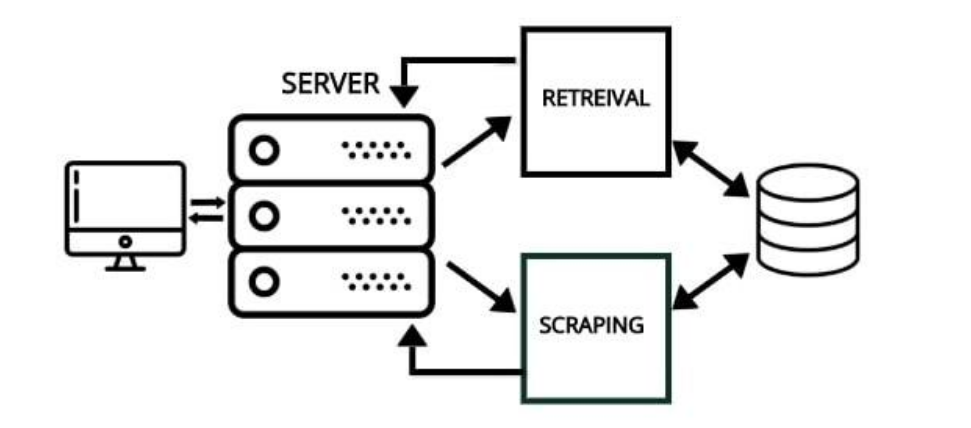
\includegraphics[width=\textwidth,height=\textheight,keepaspectratio]{../static/media/SystemArchitecture.png}
\caption{System Architecture}
\end{figure}
The figure represents the System Architecture.